%\usepackage[utf8]{inputenc}

\section{Review of (multiple) regression}
\frame{\sectionpage}




\begin{frame}{Regression}

  \begin{itemize}
  \item Use regression when one variable is an outcome ({\em response}, $y$).
  \item See if/how response depends on other variable(s), {\em explanatory}, $x_1, x_2,\ldots$.
  \item Can have {\em one} or {\em more than one} explanatory variable, but always one response.
  \item Assumes a {\em straight-line} relationship between response and explanatory.
  \item Ask: 
    \begin{itemize}
    \item {\em is there} a relationship between $y$ and $x$'s, and if so, which ones?
    \item what does the relationship look like?
    \end{itemize}

  \end{itemize}
  
\end{frame}

\begin{frame}[fragile]{A regression with one $x$}

13 children, measure average total sleep time (ATST, mins) and age (years) for each. See if ATST depends on age. Data in \verb-sleep.txt-, ATST then age. Read in data:

 
\begin{knitrout}
\definecolor{shadecolor}{rgb}{0.969, 0.969, 0.969}\color{fgcolor}\begin{kframe}
\begin{alltt}
\hlstd{sleep}\hlkwb{=}\hlkwd{read.table}\hlstd{(}\hlstr{"sleep.txt"}\hlstd{,}\hlkwc{header}\hlstd{=T)}
\hlkwd{head}\hlstd{(sleep)}
\end{alltt}
\begin{verbatim}
    atst  age
1 586.00  4.4
2 461.75 14.0
3 491.10 10.1
4 565.00  6.7
5 462.00 11.5
6 532.10  9.6
\end{verbatim}
\end{kframe}
\end{knitrout}

and make scatter plot of ATST (response) vs.\ age (explanatory) using
code overleaf:

 


\end{frame}




\begin{frame}[fragile]{The scatterplot}
   
\begin{knitrout}
\definecolor{shadecolor}{rgb}{0.969, 0.969, 0.969}\color{fgcolor}\begin{kframe}
\begin{alltt}
\hlkwd{ggplot}\hlstd{(sleep,}\hlkwd{aes}\hlstd{(}\hlkwc{x}\hlstd{=age,}\hlkwc{y}\hlstd{=atst))}\hlopt{+}\hlkwd{geom_point}\hlstd{()}
\end{alltt}
\end{kframe}
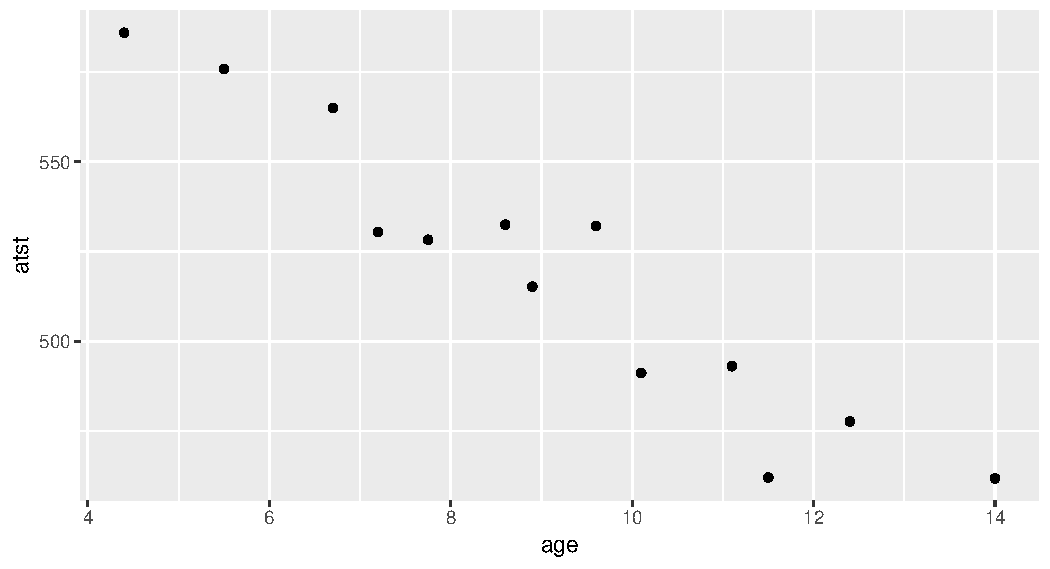
\includegraphics[width=\maxwidth]{figure/suggo-1} 

\end{knitrout}
  
  
%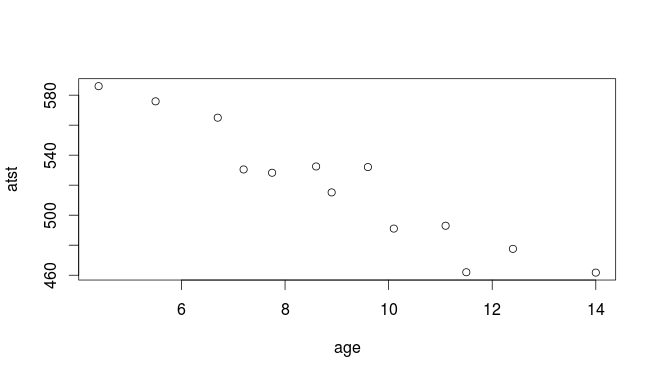
\includegraphics[width=\textwidth]{sleep-times}

\end{frame}

\begin{frame}[fragile]{Correlation}
  
  \begin{itemize}
  \item Measures how well a straight line fits the data:
 
\begin{knitrout}
\definecolor{shadecolor}{rgb}{0.969, 0.969, 0.969}\color{fgcolor}\begin{kframe}
\begin{alltt}
\hlkwd{with}\hlstd{(sleep,}\hlkwd{cor}\hlstd{(atst,age))}
\end{alltt}
\begin{verbatim}
[1] -0.9515469
\end{verbatim}
\end{kframe}
\end{knitrout}

\item $1$ is perfect upward trend, $-1$ is perfect downward trend, 0
  is no trend.
\item This one close to perfect downward trend.
\item Can do correlations of whole data frame:
 
\begin{knitrout}
\definecolor{shadecolor}{rgb}{0.969, 0.969, 0.969}\color{fgcolor}\begin{kframe}
\begin{alltt}
\hlkwd{cor}\hlstd{(sleep)}
\end{alltt}
\begin{verbatim}
           atst        age
atst  1.0000000 -0.9515469
age  -0.9515469  1.0000000
\end{verbatim}
\end{kframe}
\end{knitrout}
\item Correlations of all possible pairs of variables.  
    
  \end{itemize}
  
\end{frame}


\begin{frame}[fragile]{Lowess curve}
  
  \begin{itemize}
  \item Sometimes nice to guide the eye: is the trend straight, or not?

  \item Idea: \emph{lowess curve}. ``Locally weighted least squares'',
    not affected by outliers, not constrained to be linear.
  \item Lowess is a \emph{guide}: even if straight line appropriate,
    may wiggle/bend a little. Looking for \emph{serious} problems with
    linearity. 
  \item Add lowess curve to plot using \texttt{geom\_smooth}:
 
    
  \end{itemize}
  
\end{frame}

\begin{frame}[fragile]{Plot with lowess curve}
  

\begin{knitrout}
\definecolor{shadecolor}{rgb}{0.969, 0.969, 0.969}\color{fgcolor}\begin{kframe}
\begin{alltt}
\hlkwd{ggplot}\hlstd{(sleep,}\hlkwd{aes}\hlstd{(}\hlkwc{x}\hlstd{=age,}\hlkwc{y}\hlstd{=atst))}\hlopt{+}\hlkwd{geom_point}\hlstd{()}\hlopt{+}
  \hlkwd{geom_smooth}\hlstd{()}
\end{alltt}


{\ttfamily\noindent\itshape\color{messagecolor}{`geom\_smooth()` using method = 'loess'}}\end{kframe}
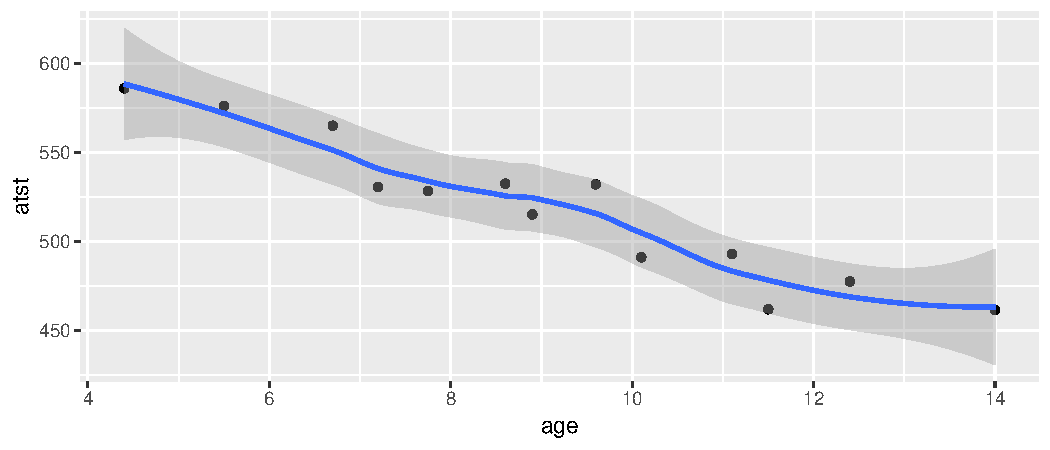
\includegraphics[width=\maxwidth]{figure/icko-1} 

\end{knitrout}

  
  
\end{frame}


\begin{frame}[fragile]{The regression}

Scatterplot shows no obvious curve, and a pretty clear downward trend. So we can run the regression:

{\scriptsize
 
\begin{knitrout}
\definecolor{shadecolor}{rgb}{0.969, 0.969, 0.969}\color{fgcolor}\begin{kframe}
\begin{alltt}
\hlstd{sleep.1}\hlkwb{=}\hlkwd{lm}\hlstd{(atst}\hlopt{~}\hlstd{age,}\hlkwc{data}\hlstd{=sleep) ;} \hlkwd{summary}\hlstd{(sleep.1)}
\end{alltt}
\begin{verbatim}

Call:
lm(formula = atst ~ age, data = sleep)

Residuals:
    Min      1Q  Median      3Q     Max 
-23.011  -9.365   2.372   6.770  20.411 

Coefficients:
            Estimate Std. Error t value Pr(>|t|)    
(Intercept)  646.483     12.918   50.05 2.49e-14 ***
age          -14.041      1.368  -10.26 5.70e-07 ***
---
Signif. codes:  
0 '***' 0.001 '**' 0.01 '*' 0.05 '.' 0.1 ' ' 1

Residual standard error: 13.15 on 11 degrees of freedom
Multiple R-squared:  0.9054,	Adjusted R-squared:  0.8968 
F-statistic: 105.3 on 1 and 11 DF,  p-value: 5.7e-07
\end{verbatim}
\end{kframe}
\end{knitrout}
}


\end{frame}

\begin{frame}{Conclusions}

    \begin{itemize}
  \item The relationship appears to be a straight line, with a downward trend.
  \item $F$-tests for model as a whole and $t$-test for slope (same)
    both confirm this (P-value $5.7\times 10^{-7}=0.00000057$).
  \item Slope is $-14$, so a 1-year increase in age goes with a 14-minute decrease in ATST on average.
  \item R-squared is correlation squared (when one $x$ anyway),
    between 0 and 1 (1 good, 0 bad).
  \item Here R-squared is 0.9054, pleasantly high.
  \end{itemize}
  
\end{frame}

% for week 2:
% 
% regression and multiple regression
% 
% including univariate + tests
% ci, pi and influential points
% multiple, re-interpretation of tests, correlated x's
% residuals and plotting
% 

% next: ci and pi with children aged 10 and 3
% then: maybe diagnostics

\begin{frame}{CI for mean response and prediction intervals}

Once useful regression exists, use it for prediction:


\begin{itemize}
\item To get a single number for prediction at a given $x$, substitute into regression equation, eg.\ age 10: predicted ATST is $646.48-14.04(10)=506$ minutes.
\item To express uncertainty of this prediction:
  \begin{itemize}
  \item {\em CI for mean response} expresses uncertainty about mean ATST for all children aged 10, based on data.
  \item {\em Prediction interval} expresses uncertainty about predicted ATST for a new child aged 10 whose ATST not known. More uncertain.
  \end{itemize}
\item Also do above for a child aged 5.
\end{itemize}
\end{frame}

\begin{frame}[fragile]{Intervals}
\begin{itemize}
\item Make new data frame with these values for \texttt{age}
\item Feed into \texttt{predict}:
  
{\small  
 
\begin{knitrout}
\definecolor{shadecolor}{rgb}{0.969, 0.969, 0.969}\color{fgcolor}\begin{kframe}
\begin{alltt}
\hlstd{my.age}\hlkwb{=}\hlkwd{c}\hlstd{(}\hlnum{10}\hlstd{,}\hlnum{5}\hlstd{)}
\hlstd{ages.new}\hlkwb{=}\hlkwd{data.frame}\hlstd{(}\hlkwc{age}\hlstd{=my.age)}
\hlstd{ages.new}
\end{alltt}
\begin{verbatim}
  age
1  10
2   5
\end{verbatim}
\begin{alltt}
\hlstd{pc}\hlkwb{=}\hlkwd{predict}\hlstd{(sleep.1,ages.new,}\hlkwc{interval}\hlstd{=}\hlstr{"c"}\hlstd{)}
\hlstd{pp}\hlkwb{=}\hlkwd{predict}\hlstd{(sleep.1,ages.new,}\hlkwc{interval}\hlstd{=}\hlstr{"p"}\hlstd{)}
\end{alltt}
\end{kframe}
\end{knitrout}
}

  
\end{itemize}

\end{frame}

\begin{frame}[fragile]{The intervals}
  
Confidence intervals for mean response:

 
\begin{knitrout}
\definecolor{shadecolor}{rgb}{0.969, 0.969, 0.969}\color{fgcolor}\begin{kframe}
\begin{alltt}
\hlkwd{cbind}\hlstd{(ages.new,pc)}
\end{alltt}
\begin{verbatim}
  age      fit      lwr      upr
1  10 506.0729 497.5574 514.5883
2   5 576.2781 561.6578 590.8984
\end{verbatim}
\end{kframe}
\end{knitrout}

Prediction intervals for new response:

 
\begin{knitrout}
\definecolor{shadecolor}{rgb}{0.969, 0.969, 0.969}\color{fgcolor}\begin{kframe}
\begin{alltt}
\hlkwd{cbind}\hlstd{(ages.new,pp)}
\end{alltt}
\begin{verbatim}
  age      fit      lwr      upr
1  10 506.0729 475.8982 536.2475
2   5 576.2781 543.8474 608.7088
\end{verbatim}
\end{kframe}
\end{knitrout}


  
\end{frame}


\begin{frame}[fragile]{Comments}

\begin{itemize}
\item Age 10 closer to centre of data, so intervals are both narrower than those for age 5.
\item Prediction intervals bigger than CI for mean (additional uncertainty).
\end{itemize}

\end{frame}


\begin{frame}[fragile]{That grey envelope}
  
\begin{knitrout}
\definecolor{shadecolor}{rgb}{0.969, 0.969, 0.969}\color{fgcolor}\begin{kframe}
\begin{alltt}
\hlstd{h5}\hlkwb{=}\hlkwd{ggplot}\hlstd{(sleep,}\hlkwd{aes}\hlstd{(}\hlkwc{x}\hlstd{=age,}\hlkwc{y}\hlstd{=atst))}\hlopt{+}\hlkwd{geom_point}\hlstd{()}\hlopt{+}
  \hlkwd{geom_smooth}\hlstd{(}\hlkwc{method}\hlstd{=}\hlstr{"lm"}\hlstd{)}\hlopt{+}
  \hlkwd{scale_y_continuous}\hlstd{(}\hlkwc{breaks}\hlstd{=}\hlkwd{seq}\hlstd{(}\hlnum{420}\hlstd{,}\hlnum{600}\hlstd{,}\hlnum{20}\hlstd{)) ; h5}
\end{alltt}
\end{kframe}
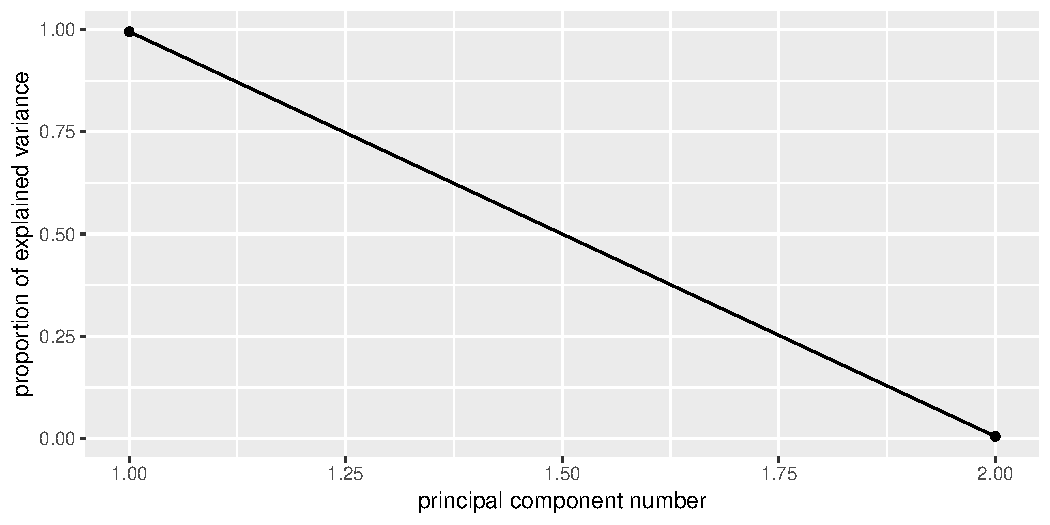
\includegraphics[width=\maxwidth]{figure/unnamed-chunk-8-1} 

\end{knitrout}

Marks confidence interval for mean for all $x$.
  
\end{frame}

\begin{frame}[fragile]{Diagnostics}
How to tell whether a straight-line regression is appropriate?

\vspace{3ex}

\begin{itemize}
\item Before: check scatterplot for straight trend.
\item After: plot {\em residuals} (observed minus predicted response) against predicted values. Aim: a plot with no pattern.
\end{itemize}

\vspace{3ex}


\end{frame}

\begin{frame}[fragile]{Output}

 
\begin{knitrout}
\definecolor{shadecolor}{rgb}{0.969, 0.969, 0.969}\color{fgcolor}\begin{kframe}
\begin{alltt}
\hlkwd{ggplot}\hlstd{(sleep.1,}\hlkwd{aes}\hlstd{(}\hlkwc{x}\hlstd{=.fitted,}\hlkwc{y}\hlstd{=.resid))}\hlopt{+}\hlkwd{geom_point}\hlstd{()}
\end{alltt}
\end{kframe}
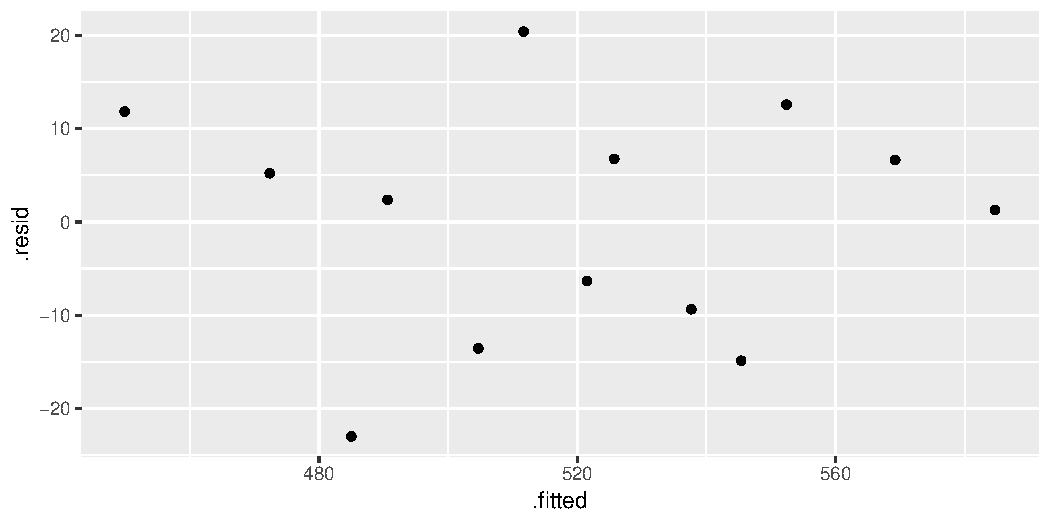
\includegraphics[width=\maxwidth]{figure/akjhkadjfhjahnkkk-1} 

\end{knitrout}
  
%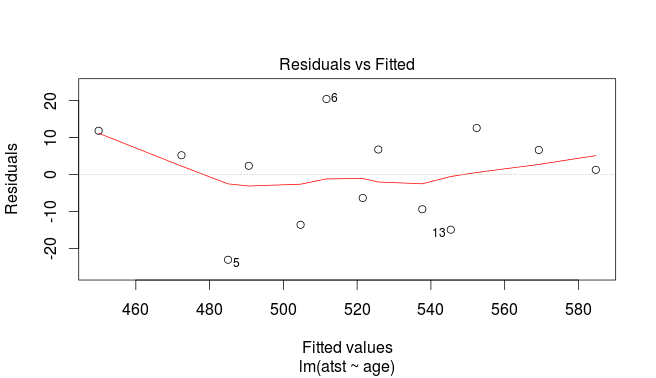
\includegraphics[width=4in]{sleep-resid}

Not much pattern here (is residual predictable from predicted? No). Good, indicating regression appropriate.
  
\end{frame}


\begin{frame}[fragile]{An inappropriate regression}

Scatterplot of different data:  
  
{\footnotesize
 
\begin{knitrout}
\definecolor{shadecolor}{rgb}{0.969, 0.969, 0.969}\color{fgcolor}\begin{kframe}
\begin{alltt}
\hlstd{curvy}\hlkwb{=}\hlkwd{read.table}\hlstd{(}\hlstr{"curvy.txt"}\hlstd{,}\hlkwc{header}\hlstd{=T)}
\hlkwd{ggplot}\hlstd{(curvy,}\hlkwd{aes}\hlstd{(}\hlkwc{x}\hlstd{=xx,}\hlkwc{y}\hlstd{=yy))}\hlopt{+}\hlkwd{geom_point}\hlstd{()}
\end{alltt}
\end{kframe}
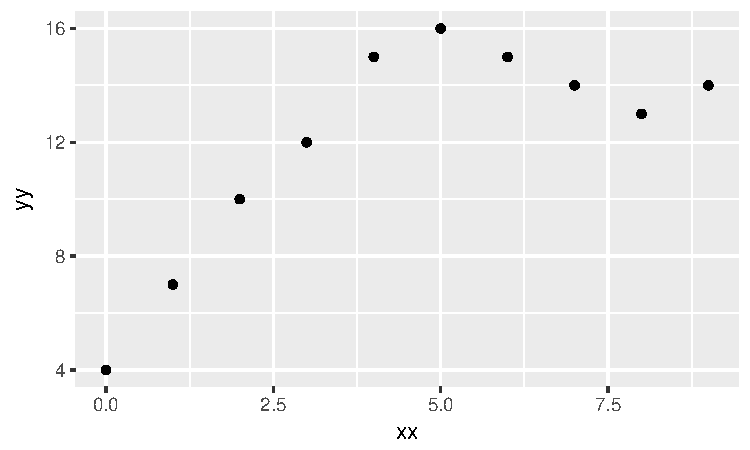
\includegraphics[width=\maxwidth]{figure/curvy-1} 

\end{knitrout}
}  
  

%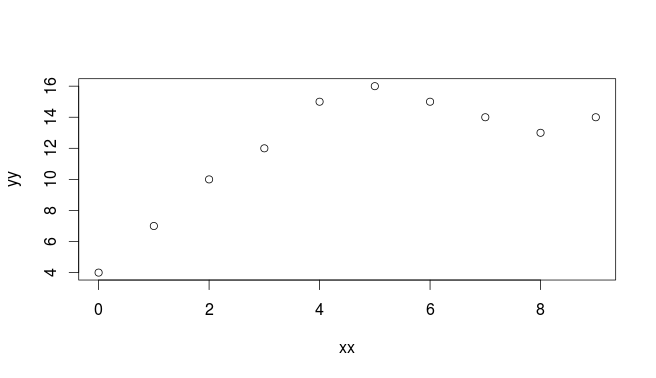
\includegraphics[width=4in]{curvy-scatter}


\end{frame}

\begin{frame}[fragile]{Regression line, anyway}

{\footnotesize
 
\begin{knitrout}
\definecolor{shadecolor}{rgb}{0.969, 0.969, 0.969}\color{fgcolor}\begin{kframe}
\begin{alltt}
\hlstd{curvy.1}\hlkwb{=}\hlkwd{lm}\hlstd{(yy}\hlopt{~}\hlstd{xx,}\hlkwc{data}\hlstd{=curvy) ;} \hlkwd{summary}\hlstd{(curvy.1)}
\end{alltt}
\begin{verbatim}

Call:
lm(formula = yy ~ xx, data = curvy)

Residuals:
   Min     1Q Median     3Q    Max 
-3.582 -2.204  0.000  1.514  3.509 

Coefficients:
            Estimate Std. Error t value Pr(>|t|)   
(Intercept)   7.5818     1.5616   4.855  0.00126 **
xx            0.9818     0.2925   3.356  0.00998 **
---
Signif. codes:  
0 '***' 0.001 '**' 0.01 '*' 0.05 '.' 0.1 ' ' 1

Residual standard error: 2.657 on 8 degrees of freedom
Multiple R-squared:  0.5848,	Adjusted R-squared:  0.5329 
F-statistic: 11.27 on 1 and 8 DF,  p-value: 0.009984
\end{verbatim}
\end{kframe}
\end{knitrout}
}
  
\end{frame}



\begin{frame}[fragile]{Residual plot}

 
\begin{knitrout}
\definecolor{shadecolor}{rgb}{0.969, 0.969, 0.969}\color{fgcolor}\begin{kframe}
\begin{alltt}
\hlkwd{ggplot}\hlstd{(curvy.1,}\hlkwd{aes}\hlstd{(}\hlkwc{x}\hlstd{=.fitted,}\hlkwc{y}\hlstd{=.resid))}\hlopt{+}\hlkwd{geom_point}\hlstd{()}
\end{alltt}
\end{kframe}
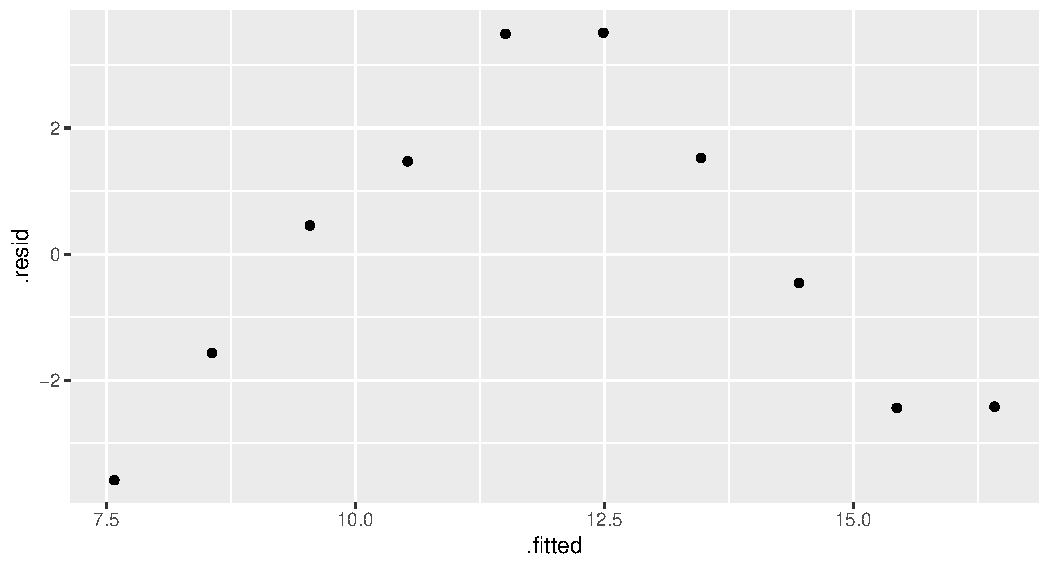
\includegraphics[width=\maxwidth]{figure/altoadige-1} 

\end{knitrout}
  
  
%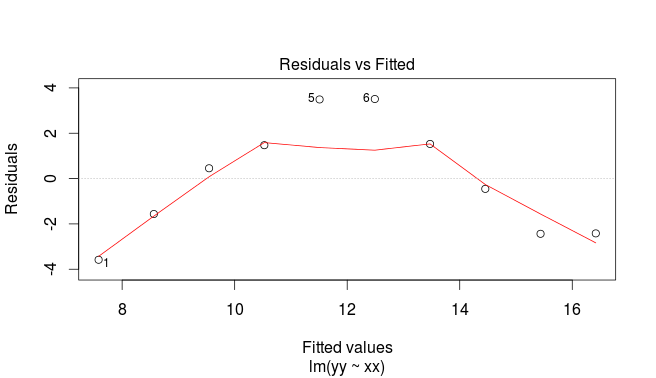
\includegraphics[width=4in]{curvy-residual}

  
\end{frame}

\begin{frame}[fragile]{No good: fixing it up}

  \begin{itemize}
  \item Residual plot has {\em curve}: middle residuals positive, high and low ones negative. Bad.
  \item Fitting a curve would be better. Try this:
  



\begin{knitrout}
\definecolor{shadecolor}{rgb}{0.969, 0.969, 0.969}\color{fgcolor}\begin{kframe}
\begin{alltt}
\hlstd{curvy.2}\hlkwb{=}\hlkwd{lm}\hlstd{(yy}\hlopt{~}\hlstd{xx}\hlopt{+}\hlkwd{I}\hlstd{(xx}\hlopt{^}\hlnum{2}\hlstd{),}\hlkwc{data}\hlstd{=curvy)}
\end{alltt}
\end{kframe}
\end{knitrout}



\item Adding \texttt{xx}-squared term, to allow for curve.
  \end{itemize}


\end{frame}



\begin{frame}[fragile]{Regression 2}
  
{\scriptsize
 
\begin{knitrout}
\definecolor{shadecolor}{rgb}{0.969, 0.969, 0.969}\color{fgcolor}\begin{kframe}
\begin{alltt}
\hlkwd{summary}\hlstd{(curvy.2)}
\end{alltt}
\begin{verbatim}

Call:
lm(formula = yy ~ xx + I(xx^2), data = curvy)

Residuals:
    Min      1Q  Median      3Q     Max 
-1.2091 -0.3602 -0.2364  0.8023  1.2636 

Coefficients:
            Estimate Std. Error t value Pr(>|t|)    
(Intercept)  3.90000    0.77312   5.045 0.001489 ** 
xx           3.74318    0.40006   9.357 3.31e-05 ***
I(xx^2)     -0.30682    0.04279  -7.170 0.000182 ***
---
Signif. codes:  
0 '***' 0.001 '**' 0.01 '*' 0.05 '.' 0.1 ' ' 1

Residual standard error: 0.9833 on 7 degrees of freedom
Multiple R-squared:  0.9502,	Adjusted R-squared:  0.936 
F-statistic: 66.83 on 2 and 7 DF,  p-value: 2.75e-05
\end{verbatim}
\end{kframe}
\end{knitrout}
  }
  
\end{frame}

\begin{frame}[fragile]{Comments}
  
  \begin{itemize}
  \item \texttt{xx}-squared term definitely significant (P-value
    0.000182), so need this curve to describe relationship.
  \item Adding squared term has made R-squared go up from 0.5848 to
    0.9502: great improvement.
  \item This is a definite curve!
  \end{itemize}
  
\end{frame}


\begin{frame}[fragile]{The residual plot now}

  
 
\begin{knitrout}
\definecolor{shadecolor}{rgb}{0.969, 0.969, 0.969}\color{fgcolor}\begin{kframe}
\begin{alltt}
\hlkwd{ggplot}\hlstd{(curvy.2,}\hlkwd{aes}\hlstd{(}\hlkwc{x}\hlstd{=.fitted,}\hlkwc{y}\hlstd{=.resid))}\hlopt{+}\hlkwd{geom_point}\hlstd{()}
\end{alltt}
\end{kframe}
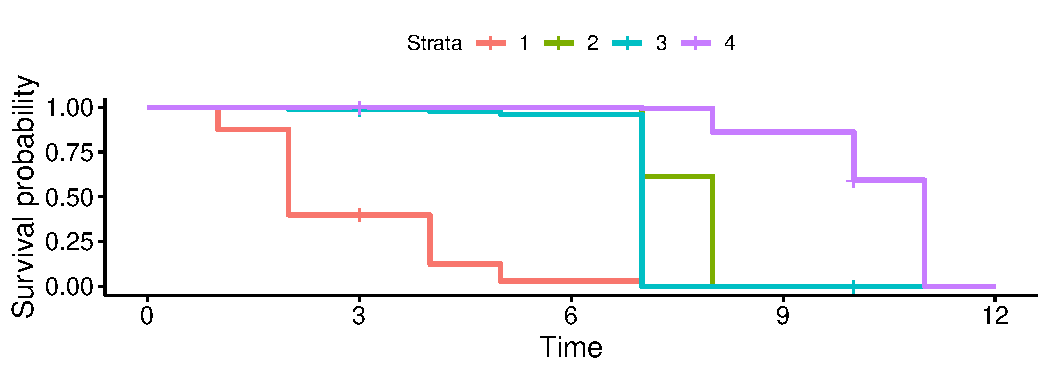
\includegraphics[width=\maxwidth]{figure/unnamed-chunk-12-1} 

\end{knitrout}

%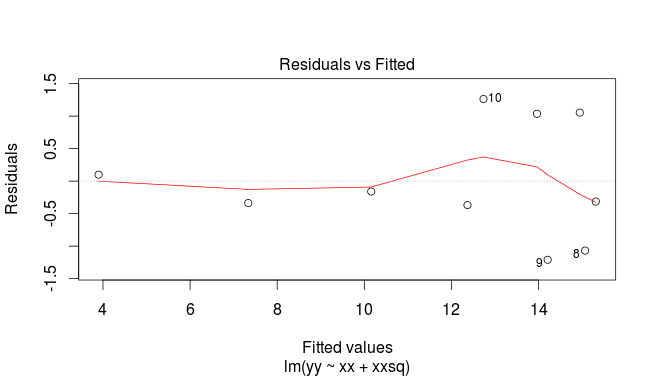
\includegraphics[width=4in]{curvy-resid2}

No problems any more.  

\end{frame}

\begin{frame}[fragile]{Another way to handle curves}
  
  \begin{itemize}
  \item Above, saw that changing $x$ (adding $x^2$) was a way of
    handling curved relationships.
  \item Another way: change $y$ (transformation).
  \item Can guess how to change $y$, or might be theory:
    \begin{itemize}
    \item example: relationship $y=ae^{bx}$ (exponential growth): 

    \item take
      logs to get $\ln y=\ln a + bx$.
    \item Taking logs has made relationship linear ($\ln y$ as response).
    \end{itemize}
  \item Or, \emph{estimate} transformation, using Box-Cox method. 
  \end{itemize}
  
\end{frame}

\begin{frame}[fragile]{Box-Cox}
  
  \begin{itemize}
  \item Install package \texttt{MASS} via
 
\begin{knitrout}
\definecolor{shadecolor}{rgb}{0.969, 0.969, 0.969}\color{fgcolor}\begin{kframe}
\begin{alltt}
\hlkwd{install.packages}\hlstd{(}\hlstr{"MASS"}\hlstd{)}
\end{alltt}
\end{kframe}
\end{knitrout}
(only need to do \emph{once})
\item Every R session you want to use something in \texttt{MASS}, type
  (no quotes)
 
\begin{knitrout}
\definecolor{shadecolor}{rgb}{0.969, 0.969, 0.969}\color{fgcolor}\begin{kframe}
\begin{alltt}
\hlkwd{library}\hlstd{(MASS)}
\end{alltt}


{\ttfamily\noindent\itshape\color{messagecolor}{\\Attaching package: 'MASS'}}

{\ttfamily\noindent\itshape\color{messagecolor}{The following object is masked from 'package:dplyr':

\ \ \ \ select}}\end{kframe}
\end{knitrout}

\end{itemize}
  
\end{frame}

\begin{frame}[fragile]{Some made-up data}
  
 
\begin{knitrout}
\definecolor{shadecolor}{rgb}{0.969, 0.969, 0.969}\color{fgcolor}\begin{kframe}
\begin{alltt}
\hlstd{madeup}\hlkwb{=}\hlkwd{read.csv}\hlstd{(}\hlstr{"madeup.csv"}\hlstd{)}
\hlstd{madeup}
\end{alltt}
\begin{verbatim}
  row x         y
1   1 0  17.92576
2   2 1  33.58480
3   3 2  82.69371
4   4 3  31.19415
5   5 4 177.07919
6   6 5 358.70001
7   7 6 469.30232
8   8 7 583.24106
\end{verbatim}
\end{kframe}
\end{knitrout}
  
Seems to be faster-than-linear growth, maybe exponential growth. Scatterplot?

 

  
\end{frame}

\begin{frame}[fragile]{The scatterplot: faster than linear growth}

  
 
\begin{knitrout}
\definecolor{shadecolor}{rgb}{0.969, 0.969, 0.969}\color{fgcolor}\begin{kframe}
\begin{alltt}
\hlkwd{ggplot}\hlstd{(madeup,}\hlkwd{aes}\hlstd{(}\hlkwc{x}\hlstd{=x,}\hlkwc{y}\hlstd{=y))}\hlopt{+}\hlkwd{geom_point}\hlstd{()}\hlopt{+}
  \hlkwd{geom_smooth}\hlstd{()}
\end{alltt}


{\ttfamily\noindent\itshape\color{messagecolor}{`geom\_smooth()` using method = 'loess'}}\end{kframe}
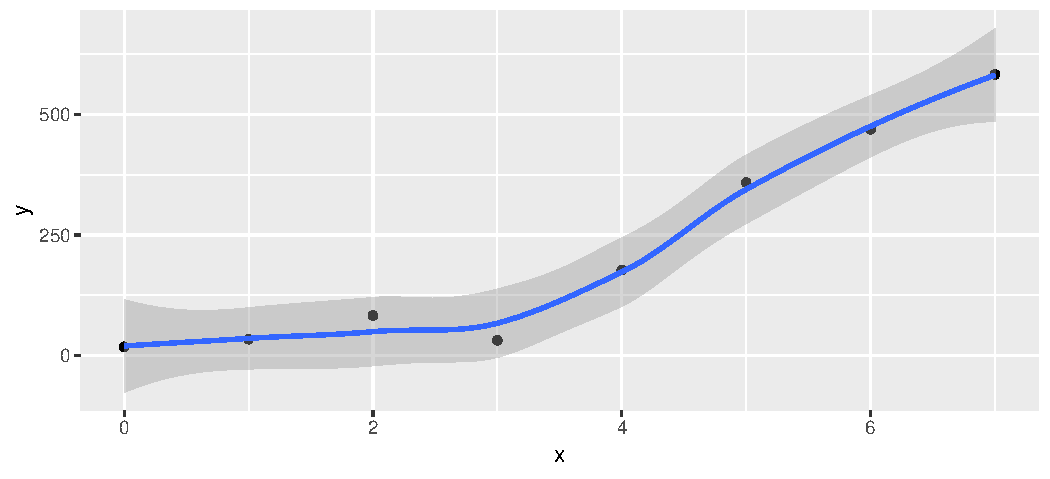
\includegraphics[width=\maxwidth]{figure/dsljhsdjlhf-1} 

\end{knitrout}

  
  
\end{frame}

\begin{frame}[fragile]{Running Box-Cox}
  
  \begin{itemize}
  \item Feed \texttt{boxcox} a model formula with a squiggle in it,
    such as you would use for \texttt{lm}.
  \item Output: a graph (next page):
 
\begin{knitrout}
\definecolor{shadecolor}{rgb}{0.969, 0.969, 0.969}\color{fgcolor}\begin{kframe}
\begin{alltt}
\hlkwd{boxcox}\hlstd{(y}\hlopt{~}\hlstd{x,}\hlkwc{data}\hlstd{=madeup)}
\end{alltt}
\end{kframe}
\end{knitrout}
    
  \end{itemize}
  
\end{frame}

\begin{frame}[fragile]{The Box-Cox output}
  
 
\begin{knitrout}
\definecolor{shadecolor}{rgb}{0.969, 0.969, 0.969}\color{fgcolor}
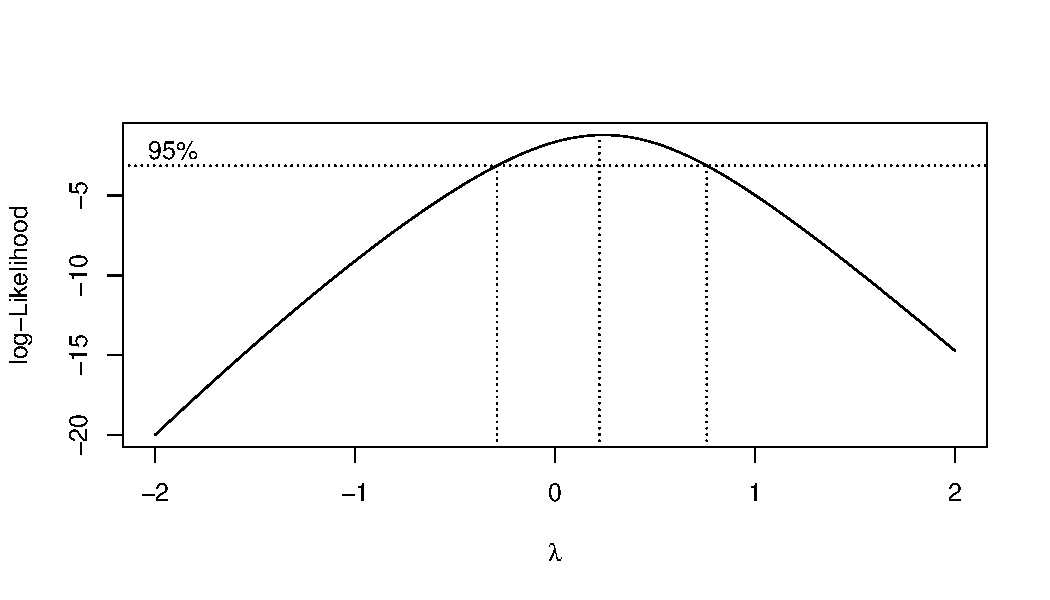
\includegraphics[width=\maxwidth]{figure/trento-1} 

\end{knitrout}
  
  
\end{frame}

\begin{frame}[fragile]{Comments}
  \begin{itemize}
  \item $\lambda$ (lambda) is the power by which you should transform
    $y$ to get the relationship straight (straighter). Power 0 is
    ``take logs''
  \item Middle dotted line marks best single value of $\lambda$ (here
    about 0.1).
  \item Outer dotted lines mark 95\% CI for $\lambda$, here $-0.3$ to
    0.7, approx. (Rather uncertain about best transformation.)
  \item Any power transformation within the CI supported by data. In
    this case, log ($\lambda=0$) and square root ($\lambda=0.5$) good,
    but no transformation ($\lambda=1$)  not.
  \item Pick a ``round-number'' value of $\lambda$ like
    $2,1,0.5,0,-0.5,-1$. Here 0 and 0.5 good values to pick. 
  \end{itemize}
\end{frame}

\begin{frame}[fragile]{Did transformation straighten things?}
  
  \begin{itemize}
  \item Calculate transformed $y$ and plot against $x$. Here try log:
 
 
\begin{knitrout}
\definecolor{shadecolor}{rgb}{0.969, 0.969, 0.969}\color{fgcolor}\begin{kframe}
\begin{alltt}
\hlstd{log.y}\hlkwb{=}\hlkwd{log}\hlstd{(madeup}\hlopt{$}\hlstd{y)}
\hlkwd{ggplot}\hlstd{(madeup,}\hlkwd{aes}\hlstd{(}\hlkwc{x}\hlstd{=x,}\hlkwc{y}\hlstd{=log.y))}\hlopt{+}\hlkwd{geom_point}\hlstd{()}\hlopt{+}
  \hlkwd{geom_smooth}\hlstd{()}
\end{alltt}


{\ttfamily\noindent\itshape\color{messagecolor}{`geom\_smooth()` using method = 'loess'}}\end{kframe}
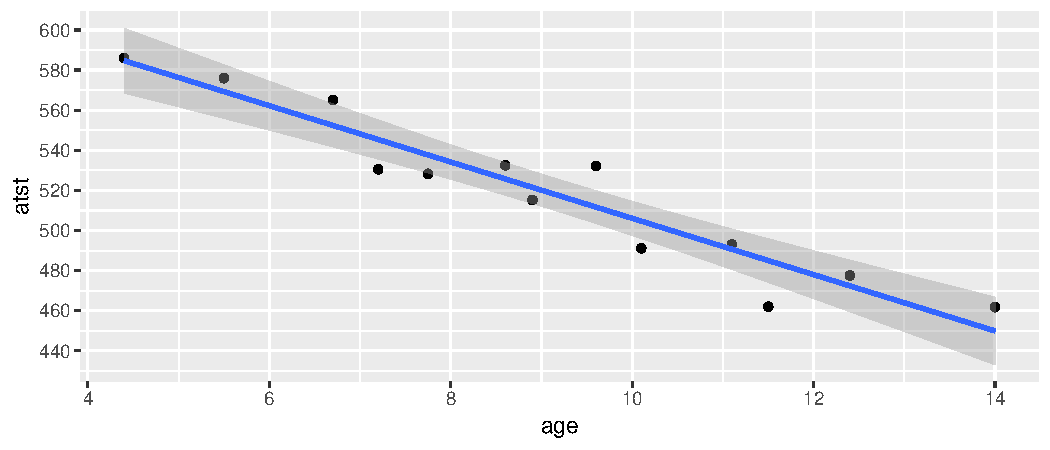
\includegraphics[width=\maxwidth]{figure/unnamed-chunk-17-1} 

\end{knitrout}

    
  \end{itemize}
  
\end{frame}

%%%%%%%%%%%%%%%%%%%%%%%%%%%%%%%%%%%%%%%%%%%%

\begin{frame}[fragile]{Multiple regression}

  \begin{itemize}
  \item What if more than one $x$? Extra issues: % regression ex from before
    \begin{itemize}
    \item Now one intercept and a slope for each $x$: how to interpret?
    \item Which $x$-variables actually help to predict $y$?

    \item Different interpretations of ``global'' $F$-test and individual $t$-tests.
    \item R-squared no longer correlation squared, but still
      interpreted as ``higher better''.
    \end{itemize}
  \item In \verb-lm- line, add extra $x$s after \verb-~-.
  \item Interpretation not so easy (and other problems that can occur).
  \end{itemize}

\end{frame}

\begin{frame}[fragile]{Multiple regression example}

Study of women and visits to health professionals, and how the number of visits might be related to other variables:

\begin{description}
\item[timedrs:] number of visits to health professionals (over course of study)
\item[phyheal:] number of physical health problems
\item[menheal:] number of mental health problems
\item[stress:] result of questionnaire about number and type of life changes
\end{description}

\verb-timedrs- response, others explanatory.

\end{frame}

\begin{frame}[fragile]{The data, fit multiple regression}

 
\begin{knitrout}
\definecolor{shadecolor}{rgb}{0.969, 0.969, 0.969}\color{fgcolor}\begin{kframe}
\begin{alltt}
\hlstd{visits}\hlkwb{=}\hlkwd{read.table}\hlstd{(}\hlstr{"regressx.txt"}\hlstd{,}\hlkwc{header}\hlstd{=T)}
\hlkwd{head}\hlstd{(visits)}
\end{alltt}
\begin{verbatim}
  subjno timedrs phyheal menheal stress
1      1       1       5       8    265
2      2       3       4       6    415
3      3       0       3       4     92
4      4      13       2       2    241
5      5      15       3       6     86
6      6       3       5       5    247
\end{verbatim}
\begin{alltt}
\hlkwd{attach}\hlstd{(visits)}
\hlstd{visits.1}\hlkwb{=}\hlkwd{lm}\hlstd{(timedrs}\hlopt{~}\hlstd{phyheal}\hlopt{+}\hlstd{menheal}\hlopt{+}\hlstd{stress)}
\end{alltt}
\end{kframe}
\end{knitrout}
  


\end{frame}

\begin{frame}[fragile]{The regression}

{\scriptsize
 
\begin{knitrout}
\definecolor{shadecolor}{rgb}{0.969, 0.969, 0.969}\color{fgcolor}\begin{kframe}
\begin{alltt}
\hlkwd{summary}\hlstd{(visits.1)}
\end{alltt}
\begin{verbatim}

Call:
lm(formula = timedrs ~ phyheal + menheal + stress)

Residuals:
    Min      1Q  Median      3Q     Max 
-14.792  -4.353  -1.815   0.902  65.886 

Coefficients:
             Estimate Std. Error t value Pr(>|t|)    
(Intercept) -3.704848   1.124195  -3.296 0.001058 ** 
phyheal      1.786948   0.221074   8.083  5.6e-15 ***
menheal     -0.009666   0.129029  -0.075 0.940318    
stress       0.013615   0.003612   3.769 0.000185 ***
---
Signif. codes:  
0 '***' 0.001 '**' 0.01 '*' 0.05 '.' 0.1 ' ' 1

Residual standard error: 9.708 on 461 degrees of freedom
Multiple R-squared:  0.2188,	Adjusted R-squared:  0.2137 
F-statistic: 43.03 on 3 and 461 DF,  p-value: < 2.2e-16
\end{verbatim}
\end{kframe}
\end{knitrout}
}  
  

\end{frame}


\begin{frame}[fragile]{The slopes}

Model as a whole strongly significant even though R-sq not very big (lots of data). At least one of the $x$'s predicts \verb-timedrs-.

\begin{footnotesize}
\begin{knitrout}
\definecolor{shadecolor}{rgb}{0.969, 0.969, 0.969}\color{fgcolor}\begin{kframe}
\begin{alltt}
\hlkwd{summary}\hlstd{(visits.1)}\hlopt{$}\hlstd{coefficients}
\end{alltt}
\begin{verbatim}
                Estimate  Std. Error     t value
(Intercept) -3.704847732 1.124195055 -3.29555598
phyheal      1.786948071 0.221073522  8.08304884
menheal     -0.009665606 0.129028610 -0.07491056
stress       0.013614518 0.003612149  3.76909138
                Pr(>|t|)
(Intercept) 1.058053e-03
phyheal     5.604170e-15
menheal     9.403184e-01
stress      1.851166e-04
\end{verbatim}
\end{kframe}
\end{knitrout}
  
\end{footnotesize}

The physical health and stress variables definitely help to predict the number of visits, but {\em with those in the model} we don't need \verb-menheal-.


However, look at prediction of \verb-timedrs- from \verb-menheal- by itself:
  
\end{frame}

\begin{frame}[fragile]{Just \texttt{menheal}}

{\footnotesize 
 
\begin{knitrout}
\definecolor{shadecolor}{rgb}{0.969, 0.969, 0.969}\color{fgcolor}\begin{kframe}
\begin{alltt}
\hlstd{visits.2}\hlkwb{=}\hlkwd{lm}\hlstd{(timedrs}\hlopt{~}\hlstd{menheal) ;} \hlkwd{summary}\hlstd{(visits.2)}
\end{alltt}
\begin{verbatim}

Call:
lm(formula = timedrs ~ menheal)

Residuals:
    Min      1Q  Median      3Q     Max 
-13.826  -5.150  -2.818   1.177  72.513 

Coefficients:
            Estimate Std. Error t value Pr(>|t|)    
(Intercept)   3.8159     0.8702   4.385 1.44e-05 ***
menheal       0.6672     0.1173   5.688 2.28e-08 ***
---
Signif. codes:  
0 '***' 0.001 '**' 0.01 '*' 0.05 '.' 0.1 ' ' 1

Residual standard error: 10.6 on 463 degrees of freedom
Multiple R-squared:  0.06532,	Adjusted R-squared:  0.0633 
F-statistic: 32.35 on 1 and 463 DF,  p-value: 2.279e-08
\end{verbatim}
\end{kframe}
\end{knitrout}
}

\end{frame}

\begin{frame}[fragile]{\texttt{menheal} by itself}

  \begin{itemize}
  \item \verb-menheal- by itself {\em does} significantly help to predict \verb-timedrs-.
  \item But the R-sq is much less (6.5\% vs.\ 22\%).
  \item So other two variables do a better job of prediction.
  \item With those variables in the regression (\texttt{phyheal} and
    \texttt{stress}), don't need \texttt{menheal} \emph{as well}.

  \end{itemize}
  


  
\end{frame}





\begin{frame}[fragile]{Investigating via correlation}
  
Leave out first column (\texttt{subjno}):
  
 
\begin{knitrout}
\definecolor{shadecolor}{rgb}{0.969, 0.969, 0.969}\color{fgcolor}\begin{kframe}
\begin{alltt}
\hlkwd{cor}\hlstd{(visits[,}\hlopt{-}\hlnum{1}\hlstd{])}
\end{alltt}
\begin{verbatim}
          timedrs   phyheal   menheal    stress
timedrs 1.0000000 0.4395293 0.2555703 0.2865951
phyheal 0.4395293 1.0000000 0.5049464 0.3055517
menheal 0.2555703 0.5049464 1.0000000 0.3697911
stress  0.2865951 0.3055517 0.3697911 1.0000000
\end{verbatim}
\end{kframe}
\end{knitrout}
  
\begin{itemize}
\item \texttt{phyheal} most strongly correlated with \texttt{timedrs}.
\item Not much to choose between other two.
\item But \texttt{menheal} has higher correlation with \texttt{phyheal},
  so not as much to \emph{add} to prediction as \texttt{stress}.
\item Goes to show things more complicated in multiple regression.

\end{itemize}

  
\end{frame}

\begin{frame}[fragile]{Residual plot (from \texttt{timedrs} on all)}
 
\begin{knitrout}
\definecolor{shadecolor}{rgb}{0.969, 0.969, 0.969}\color{fgcolor}\begin{kframe}
\begin{alltt}
\hlkwd{ggplot}\hlstd{(visits.1,}\hlkwd{aes}\hlstd{(}\hlkwc{x}\hlstd{=.fitted,}\hlkwc{y}\hlstd{=.resid))}\hlopt{+}\hlkwd{geom_point}\hlstd{()}
\end{alltt}
\end{kframe}
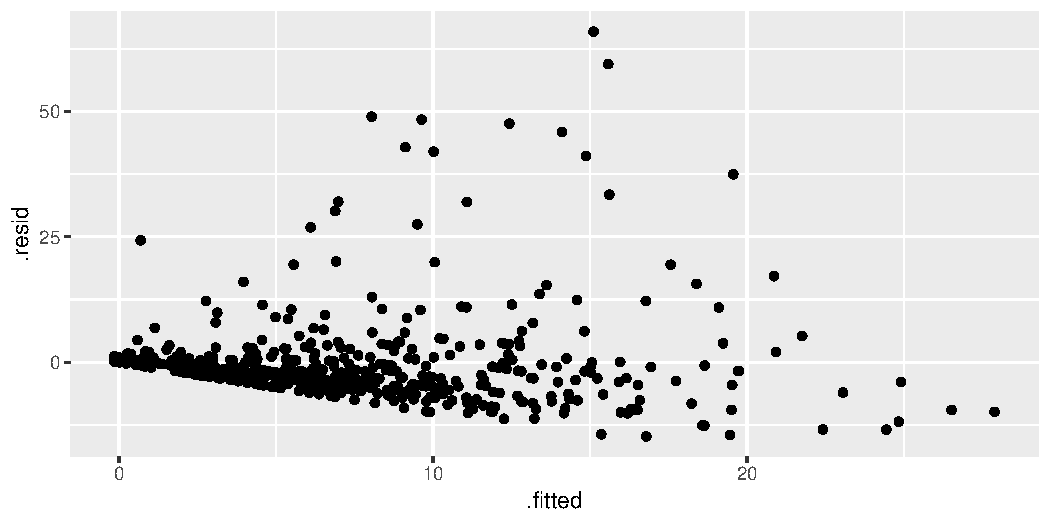
\includegraphics[width=\maxwidth]{figure/iffy8-1} 

\end{knitrout}

Apparently random. But look at all output from \texttt{plot(visits.1)}:

%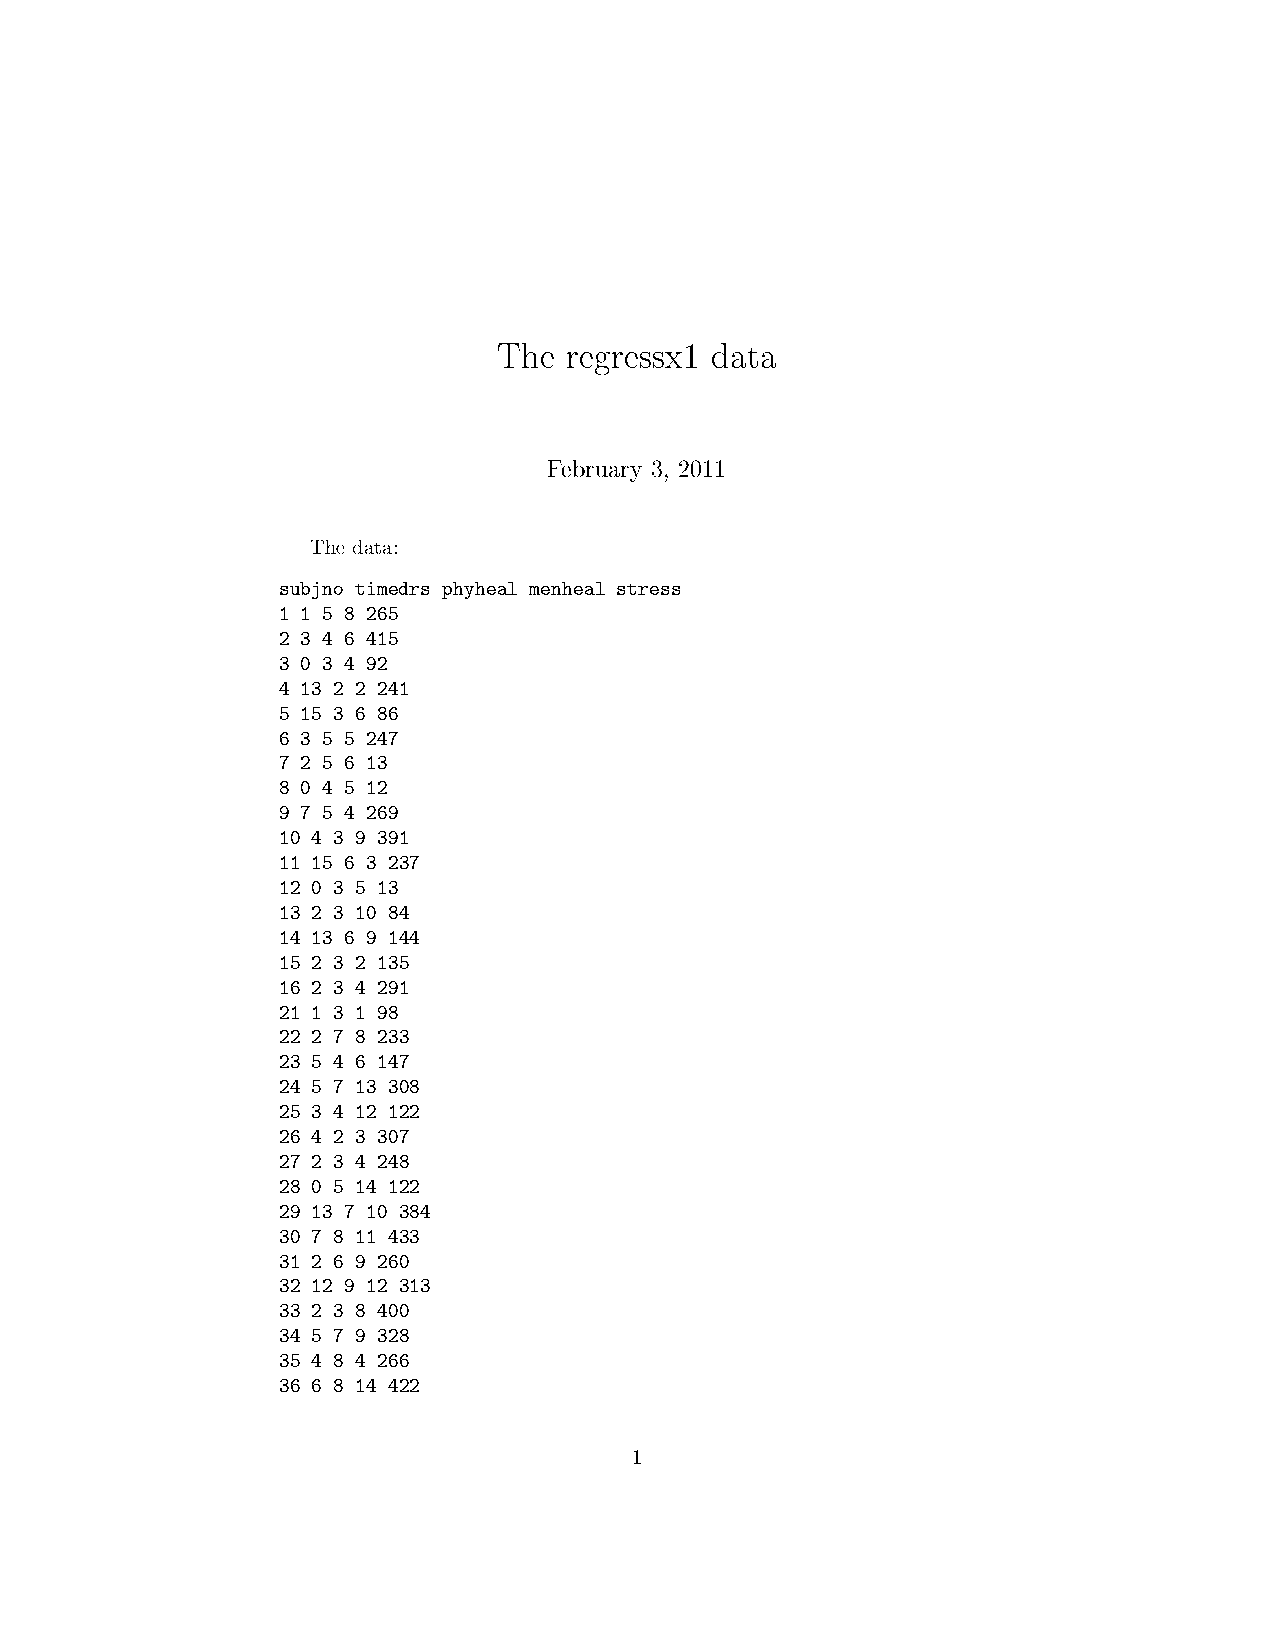
\includegraphics[width=4in]{regressx1}

\end{frame}

\begin{frame}[fragile]{Plot of regression object}
  
  
 
\begin{knitrout}
\definecolor{shadecolor}{rgb}{0.969, 0.969, 0.969}\color{fgcolor}\begin{kframe}
\begin{alltt}
\hlkwd{par}\hlstd{(}\hlkwc{mfrow}\hlstd{=}\hlkwd{c}\hlstd{(}\hlnum{2}\hlstd{,}\hlnum{2}\hlstd{)) ;} \hlkwd{plot}\hlstd{(visits.1)}
\end{alltt}
\end{kframe}
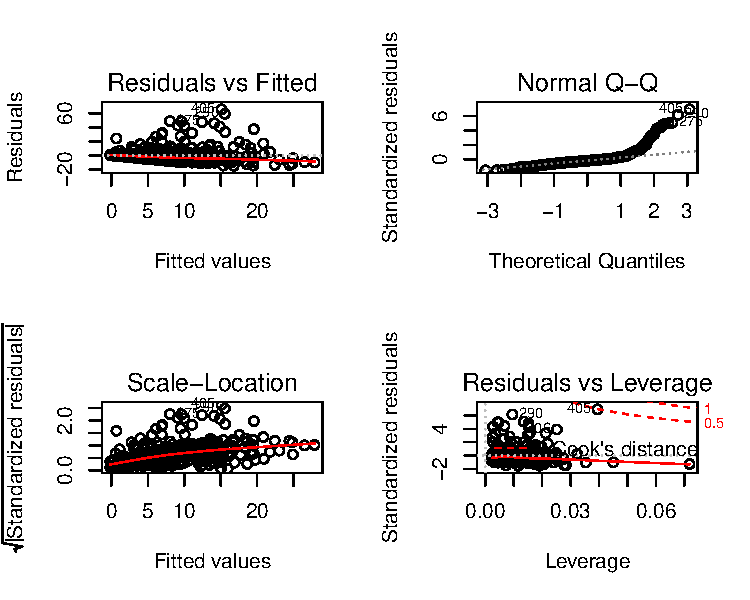
\includegraphics[width=\maxwidth]{figure/dawlish-1} 

\end{knitrout}
  
  
\end{frame}

\begin{frame}[fragile]{What are those plots?}
  
  \begin{itemize}
  \item Top left: ordinary residual plot
    \begin{itemize}
    \item no apparent pattern here
    \end{itemize}
  \item Top right: normal quantile plot of residuals
    \begin{itemize}
    \item residuals should be normally distributed
    \item should follow dotted line
    \item largest (positive) residuals are much too big
    \end{itemize}
  \item Bottom left: \emph{size} of residuals
    \begin{itemize}
    \item should stay constant
    \item here seems to be increasing: ``fan out''.
    \end{itemize}
  \item Bottom right: unusual/influential observations
    \begin{itemize}
    \item Obs at 0.07 on $x$ scale has unusual combo of $x$'s
    \item Obs 405 (top) influential over slopes.
    \end{itemize}
  \end{itemize}
  
\end{frame}


\begin{frame}[fragile]{Fixing the problems}

  \begin{itemize}
  \item Residuals not normal (skewed right), increase in size with
    fitted value.
  \item Sometimes residuals are {\em very} positive: observed a {\em lot} larger than predicted.
  \item Try {\em  transforming} response: use log or square root of response. (Note that response is {\em count}, often skewed to right.)
  \item Try regression again, with transformed response instead of
    original one.
  \item Then check residual plot to see that it is OK now.

 
\begin{knitrout}
\definecolor{shadecolor}{rgb}{0.969, 0.969, 0.969}\color{fgcolor}\begin{kframe}
\begin{alltt}
\hlstd{lgtime}\hlkwb{=}\hlkwd{log}\hlstd{(timedrs}\hlopt{+}\hlnum{1}\hlstd{)}
\hlstd{visits.3}\hlkwb{=}\hlkwd{lm}\hlstd{(lgtime}\hlopt{~}\hlstd{phyheal}\hlopt{+}\hlstd{menheal}\hlopt{+}\hlstd{stress)}
\end{alltt}
\end{kframe}
\end{knitrout}
    
\item \texttt{timedrs+1}  because some \texttt{timedrs} values 0,
  can't take log of 0.
  \end{itemize}
  
\end{frame}


\begin{frame}[fragile]{Output}

{\scriptsize
 
\begin{knitrout}
\definecolor{shadecolor}{rgb}{0.969, 0.969, 0.969}\color{fgcolor}\begin{kframe}
\begin{alltt}
\hlkwd{summary}\hlstd{(visits.3)}
\end{alltt}
\begin{verbatim}

Call:
lm(formula = lgtime ~ phyheal + menheal + stress)

Residuals:
     Min       1Q   Median       3Q      Max 
-1.95865 -0.44076 -0.02331  0.42304  2.36797 

Coefficients:
             Estimate Std. Error t value Pr(>|t|)    
(Intercept) 0.3903862  0.0882908   4.422 1.22e-05 ***
phyheal     0.2019361  0.0173624  11.631  < 2e-16 ***
menheal     0.0071442  0.0101335   0.705    0.481    
stress      0.0013158  0.0002837   4.638 4.58e-06 ***
---
Signif. codes:  
0 '***' 0.001 '**' 0.01 '*' 0.05 '.' 0.1 ' ' 1

Residual standard error: 0.7625 on 461 degrees of freedom
Multiple R-squared:  0.3682,	Adjusted R-squared:  0.3641 
F-statistic: 89.56 on 3 and 461 DF,  p-value: < 2.2e-16
\end{verbatim}
\end{kframe}
\end{knitrout}
}
 
\end{frame}

\begin{frame}[fragile]{Comments}

  \begin{itemize}
  \item Model as a whole strongly significant again 
  \item R-sq higher than before (37\% vs.\ 22\%) suggesting things more linear now
  \item Same conclusion re \verb-menheal-: can take out of regression.
  \item Should look at residual plots (next page).
  \end{itemize}
  
\end{frame}

\begin{frame}[fragile]{The residual plots}

 
\begin{knitrout}
\definecolor{shadecolor}{rgb}{0.969, 0.969, 0.969}\color{fgcolor}\begin{kframe}
\begin{alltt}
\hlkwd{par}\hlstd{(}\hlkwc{mfrow}\hlstd{=}\hlkwd{c}\hlstd{(}\hlnum{2}\hlstd{,}\hlnum{2}\hlstd{)) ;} \hlkwd{plot}\hlstd{(visits.3)}
\end{alltt}
\end{kframe}
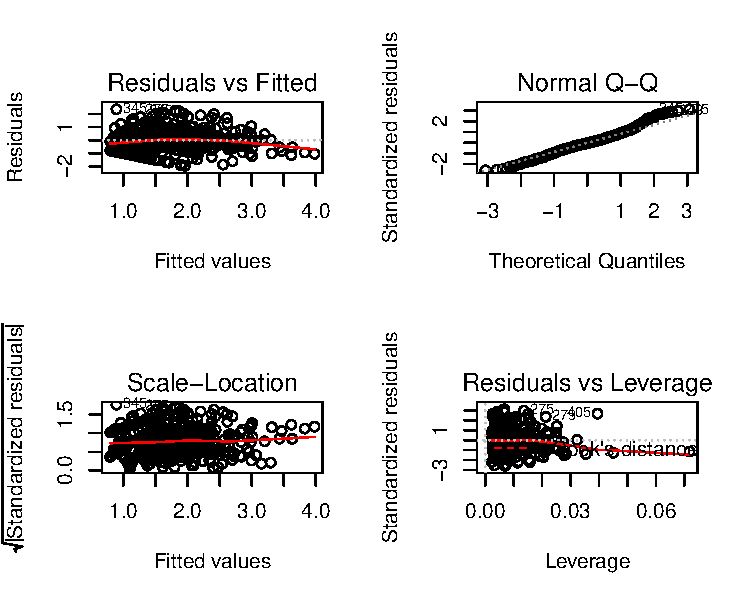
\includegraphics[width=\maxwidth]{figure/asljsakjhd-1} 

\end{knitrout}
  
  
\end{frame}

\begin{frame}[fragile]{Comments}

  
  \begin{itemize}
  \item Residuals range from about 2 to $-2$.
  \item Residuals look much more normally distributed.
  \item Size of residuals (bottom left) doesn't seem to change much.
  \item Much better now.
  \end{itemize}
  
  
\end{frame}

\begin{frame}[fragile]{Box-Cox transformations}


  \begin{itemize}
  \item Taking log of \verb-timedrs- and having it work: lucky
    guess. How to find good transformation?
  \item Box-Cox again.
  \item Extra problem: some of \verb-timedrs- values are 0, but Box-Cox expects all
    +. Note extra step in defining \texttt{tp}:

 
\begin{knitrout}
\definecolor{shadecolor}{rgb}{0.969, 0.969, 0.969}\color{fgcolor}\begin{kframe}
\begin{alltt}
\hlstd{tp}\hlkwb{=}\hlstd{timedrs}\hlopt{+}\hlnum{1}
\hlkwd{library}\hlstd{(MASS)}
\end{alltt}
\end{kframe}
\end{knitrout}
    
 
\begin{knitrout}
\definecolor{shadecolor}{rgb}{0.969, 0.969, 0.969}\color{fgcolor}\begin{kframe}
\begin{alltt}
\hlkwd{boxcox}\hlstd{(tp}\hlopt{~}\hlstd{phyheal}\hlopt{+}\hlstd{menheal}\hlopt{+}\hlstd{stress)}
\end{alltt}
\end{kframe}
\end{knitrout}
  \end{itemize}

\end{frame}


\begin{frame}[fragile]{Try 1}

 
\begin{knitrout}
\definecolor{shadecolor}{rgb}{0.969, 0.969, 0.969}\color{fgcolor}
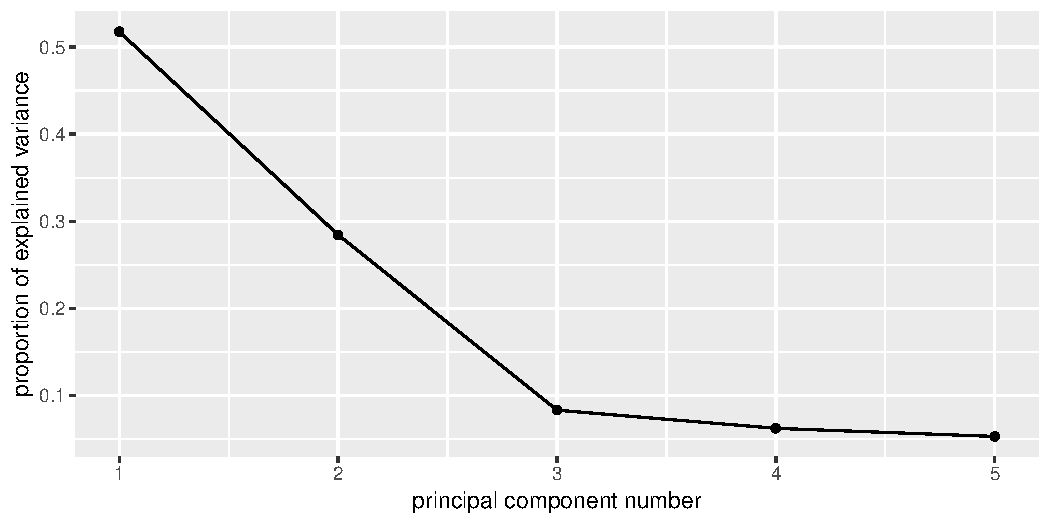
\includegraphics[width=\maxwidth]{figure/unnamed-chunk-27-1} 

\end{knitrout}
  
  
\end{frame}

\begin{frame}[fragile]{Comments on try 1}

  \begin{itemize}
\item Best: $\lambda$ just less than zero.
\item Hard to see scale. 
\item Focus on $\lambda$ in $(-0.3,0.1)$:
{\small    
 
\begin{knitrout}
\definecolor{shadecolor}{rgb}{0.969, 0.969, 0.969}\color{fgcolor}\begin{kframe}
\begin{alltt}
\hlstd{my.lambda}\hlkwb{=}\hlkwd{seq}\hlstd{(}\hlopt{-}\hlnum{0.3}\hlstd{,}\hlnum{0.1}\hlstd{,}\hlnum{0.01}\hlstd{)}
\hlstd{my.lambda}
\end{alltt}
\begin{verbatim}
 [1] -0.30 -0.29 -0.28 -0.27 -0.26 -0.25 -0.24 -0.23 -0.22
[10] -0.21 -0.20 -0.19 -0.18 -0.17 -0.16 -0.15 -0.14 -0.13
[19] -0.12 -0.11 -0.10 -0.09 -0.08 -0.07 -0.06 -0.05 -0.04
[28] -0.03 -0.02 -0.01  0.00  0.01  0.02  0.03  0.04  0.05
[37]  0.06  0.07  0.08  0.09  0.10
\end{verbatim}
\end{kframe}
\end{knitrout}
}


\end{itemize}

  
  
\end{frame}




\begin{frame}[fragile]{Try 2}

 
\begin{knitrout}
\definecolor{shadecolor}{rgb}{0.969, 0.969, 0.969}\color{fgcolor}\begin{kframe}
\begin{alltt}
\hlkwd{boxcox}\hlstd{(tp}\hlopt{~}\hlstd{phyheal}\hlopt{+}\hlstd{menheal}\hlopt{+}\hlstd{stress,}\hlkwc{lambda}\hlstd{=my.lambda)}
\end{alltt}
\end{kframe}
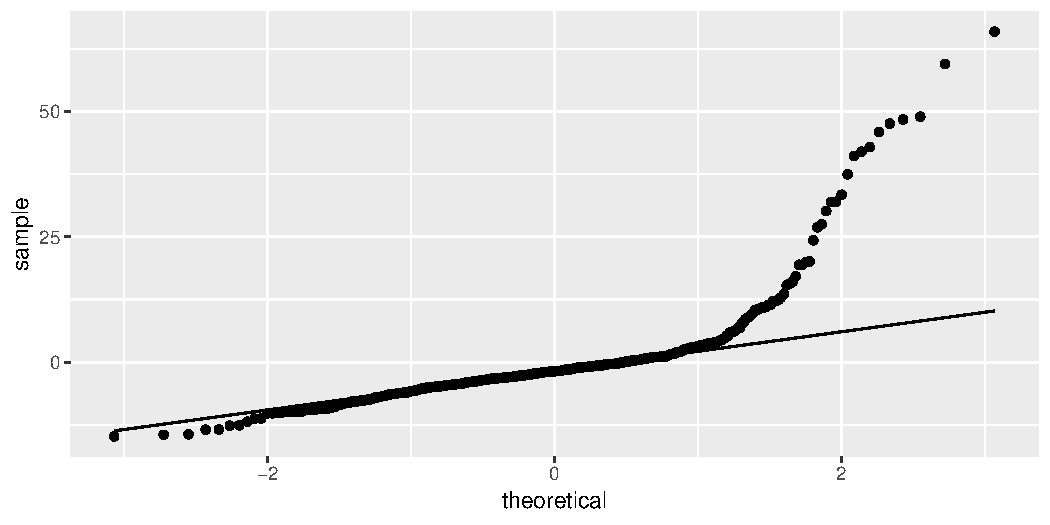
\includegraphics[width=\maxwidth]{figure/unnamed-chunk-29-1} 

\end{knitrout}

  

\end{frame}

\begin{frame}[fragile]{Comments}
  
\begin{itemize}
\item Best: $\lambda$ just about $-0.07$.
\item CI for $\lambda$ about $(-0.14,0.01)$.
\item Only nearby round number: $\lambda=0$, log transformation.
\item So we made lucky guess with log before!
\end{itemize}
  
  
\end{frame}


\begin{frame}[fragile]{Testing more than one $x$ at once}

The $t$-tests test only whether one variable could be taken out of the
regression you're looking at. To test significance of more than one
variable at once, fit model with and without variables and use
\texttt{anova} to compare fit of models:


{\small
\begin{knitrout}
\definecolor{shadecolor}{rgb}{0.969, 0.969, 0.969}\color{fgcolor}\begin{kframe}
\begin{alltt}
\hlstd{visits.5}\hlkwb{=}\hlkwd{lm}\hlstd{(lgtime}\hlopt{~}\hlstd{phyheal}\hlopt{+}\hlstd{menheal}\hlopt{+}\hlstd{stress)}
\hlstd{visits.6}\hlkwb{=}\hlkwd{lm}\hlstd{(lgtime}\hlopt{~}\hlstd{stress)}
\hlkwd{anova}\hlstd{(visits.6,visits.5)}
\end{alltt}
\begin{verbatim}
Analysis of Variance Table

Model 1: lgtime ~ stress
Model 2: lgtime ~ phyheal + menheal + stress
  Res.Df    RSS Df Sum of Sq      F    Pr(>F)    
1    463 371.47                                  
2    461 268.01  2    103.46 88.984 < 2.2e-16 ***
---
Signif. codes:  
0 '***' 0.001 '**' 0.01 '*' 0.05 '.' 0.1 ' ' 1
\end{verbatim}
\end{kframe}
\end{knitrout}
}


\end{frame}

\begin{frame}[fragile]{Results of tests}


\begin{itemize}

\item Models don't fit equally well, so big one fits better.
\item Or ``taking both variables out makes the fit worse, so don't do it''.
\item   Taking out those $x$'s
  is a mistake. Or putting them in is a good idea.
\end{itemize}
  
\end{frame}

\begin{frame}[fragile]{The punting data}

  Data set \verb-punting.dat- contains 4 variables for 13 right-footed
  football kickers (punters): left leg and right leg strength (lbs),
  distance punted (ft), another variable called ``fred''. Predict
  punting distance from other variables:

 
\begin{knitrout}
\definecolor{shadecolor}{rgb}{0.969, 0.969, 0.969}\color{fgcolor}\begin{kframe}
\begin{alltt}
\hlstd{punting}\hlkwb{=}\hlkwd{read.table}\hlstd{(}\hlstr{"punting.txt"}\hlstd{,}\hlkwc{header}\hlstd{=T)}
\hlkwd{head}\hlstd{(punting)}
\end{alltt}
\begin{verbatim}
  left right   punt fred
1  170   170 162.50  171
2  130   140 144.00  136
3  170   180 174.50  174
4  160   160 163.50  161
5  150   170 192.00  159
6  150   150 171.75  151
\end{verbatim}
\begin{alltt}
\hlkwd{attach}\hlstd{(punting)}
\hlstd{punting.1}\hlkwb{=}\hlkwd{lm}\hlstd{(punt}\hlopt{~}\hlstd{left}\hlopt{+}\hlstd{right}\hlopt{+}\hlstd{fred)}
\end{alltt}
\end{kframe}
\end{knitrout}
  
  
\end{frame}

\begin{frame}[fragile]{Regression output}

{\small
 
\begin{knitrout}
\definecolor{shadecolor}{rgb}{0.969, 0.969, 0.969}\color{fgcolor}\begin{kframe}
\begin{alltt}
\hlkwd{summary}\hlstd{(punting.1)}
\end{alltt}
\begin{verbatim}

Call:
lm(formula = punt ~ left + right + fred)

Residuals:
     Min       1Q   Median       3Q      Max 
-14.9325 -11.5618  -0.0315   9.0415  20.0886 

Coefficients:
            Estimate Std. Error t value Pr(>|t|)
(Intercept)  -4.6855    29.1172  -0.161    0.876
left          0.2679     2.1111   0.127    0.902
right         1.0524     2.1477   0.490    0.636
fred         -0.2672     4.2266  -0.063    0.951

Residual standard error: 14.68 on 9 degrees of freedom
Multiple R-squared:  0.7781,	Adjusted R-squared:  0.7042 
F-statistic: 10.52 on 3 and 9 DF,  p-value: 0.00267
\end{verbatim}
\end{kframe}
\end{knitrout}
}


\end{frame}


\begin{frame}{Comments}

  \begin{itemize}
  \item Overall regression strongly significant, R-sq high.
  \item None of the $x$'s significant! Why?
  \item $t$-tests only say that you could take any one of the $x$'s out without damaging the fit; doesn't matter which one.
  \item Explanation: look at {\em correlations}. 
  \end{itemize}
\end{frame}

\begin{frame}[fragile]{The correlations}  

 
\begin{knitrout}
\definecolor{shadecolor}{rgb}{0.969, 0.969, 0.969}\color{fgcolor}\begin{kframe}
\begin{alltt}
\hlkwd{cor}\hlstd{(punting)}
\end{alltt}
\begin{verbatim}
           left     right      punt      fred
left  1.0000000 0.8957224 0.8117368 0.9722632
right 0.8957224 1.0000000 0.8805469 0.9728784
punt  0.8117368 0.8805469 1.0000000 0.8679507
fred  0.9722632 0.9728784 0.8679507 1.0000000
\end{verbatim}
\end{kframe}
\end{knitrout}
  

\begin{itemize}
\item {\em All} correlations are high: $x$'s with \verb-punt- (good) and
with each other (bad, at least confusing).
\item What to do? Probably do just as well to pick one variable, say
\texttt{right} since kickers are right-footed.
\end{itemize}



\end{frame}

\begin{frame}[fragile]{Just \texttt{right}}

  {\small
 
\begin{knitrout}
\definecolor{shadecolor}{rgb}{0.969, 0.969, 0.969}\color{fgcolor}\begin{kframe}
\begin{alltt}
\hlstd{punting.2}\hlkwb{=}\hlkwd{lm}\hlstd{(punt}\hlopt{~}\hlstd{right)}
\hlkwd{anova}\hlstd{(punting.2,punting.1)}
\end{alltt}
\begin{verbatim}
Analysis of Variance Table

Model 1: punt ~ right
Model 2: punt ~ left + right + fred
  Res.Df    RSS Df Sum of Sq      F Pr(>F)
1     11 1962.5                           
2      9 1938.2  2    24.263 0.0563 0.9456
\end{verbatim}
\end{kframe}
\end{knitrout}
}
  

No significant loss by dropping other two variables.

\end{frame}

\begin{frame}[fragile]{Comparing R-squareds}


{\small
\begin{knitrout}
\definecolor{shadecolor}{rgb}{0.969, 0.969, 0.969}\color{fgcolor}\begin{kframe}
\begin{alltt}
\hlkwd{summary}\hlstd{(punting.1)}\hlopt{$}\hlstd{r.squared}
\end{alltt}
\begin{verbatim}
[1] 0.7781401
\end{verbatim}
\begin{alltt}
\hlkwd{summary}\hlstd{(punting.2)}\hlopt{$}\hlstd{r.squared}
\end{alltt}
\begin{verbatim}
[1] 0.7753629
\end{verbatim}
\end{kframe}
\end{knitrout}
}

Basically no difference. In regression (over), \texttt{right} significant:
  

  
\end{frame}

\begin{frame}[fragile]{Regression results}

{\footnotesize
 
\begin{knitrout}
\definecolor{shadecolor}{rgb}{0.969, 0.969, 0.969}\color{fgcolor}\begin{kframe}
\begin{alltt}
\hlkwd{summary}\hlstd{(punting.2)}
\end{alltt}
\begin{verbatim}

Call:
lm(formula = punt ~ right)

Residuals:
     Min       1Q   Median       3Q      Max 
-15.7576 -11.0611   0.3656   7.8890  19.0423 

Coefficients:
            Estimate Std. Error t value Pr(>|t|)    
(Intercept)  -3.6930    25.2649  -0.146    0.886    
right         1.0427     0.1692   6.162 7.09e-05 ***
---
Signif. codes:  
0 '***' 0.001 '**' 0.01 '*' 0.05 '.' 0.1 ' ' 1

Residual standard error: 13.36 on 11 degrees of freedom
Multiple R-squared:  0.7754,	Adjusted R-squared:  0.7549 
F-statistic: 37.97 on 1 and 11 DF,  p-value: 7.088e-05
\end{verbatim}
\end{kframe}
\end{knitrout}
}
 
\end{frame}


\begin{frame}[fragile]{But\ldots}
  
  \begin{itemize}
  \item Maybe we got the \emph{form} of the relationship with
    \texttt{left} wrong.
  \item Check: plot \emph{residuals} from previous regression (without
    \texttt{left}) against \texttt{left}.
  \item Residuals here are ``punting distance adjusted for right
    leg strength''.
  \item If there is some kind of relationship with \texttt{left}, we
    should include in model.
  \end{itemize}
  
\end{frame}

\begin{frame}[fragile]{Residuals against \texttt{left}}
  
\begin{knitrout}
\definecolor{shadecolor}{rgb}{0.969, 0.969, 0.969}\color{fgcolor}\begin{kframe}
\begin{alltt}
\hlstd{r}\hlkwb{=}\hlkwd{resid}\hlstd{(punting.2)}
\hlkwd{ggplot}\hlstd{(punting,}\hlkwd{aes}\hlstd{(}\hlkwc{x}\hlstd{=left,}\hlkwc{y}\hlstd{=r))}\hlopt{+}\hlkwd{geom_point}\hlstd{()}\hlopt{+}\hlkwd{geom_smooth}\hlstd{()}
\end{alltt}


{\ttfamily\noindent\itshape\color{messagecolor}{`geom\_smooth()` using method = 'loess'}}\end{kframe}
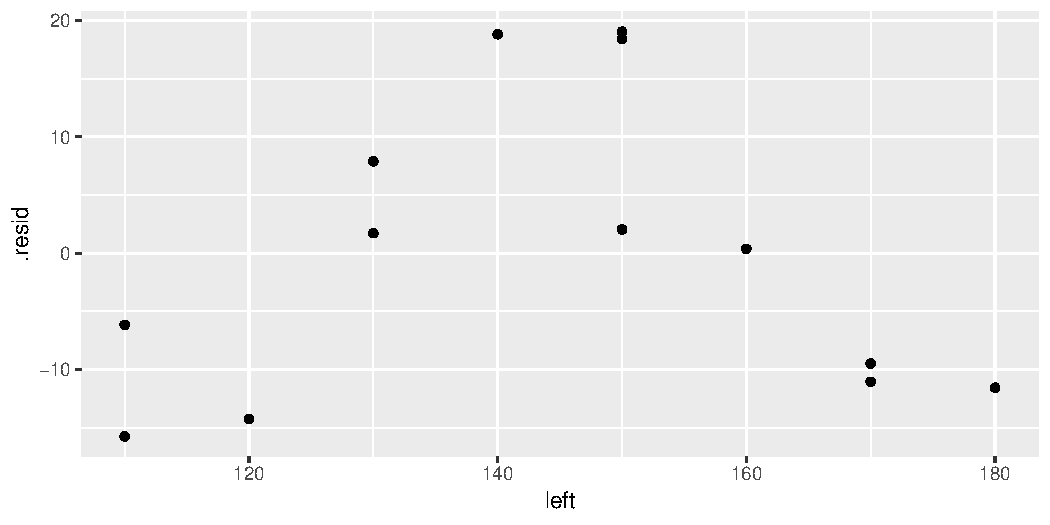
\includegraphics[width=\maxwidth]{figure/basingstoke-1} 

\end{knitrout}
  
\end{frame}

\begin{frame}[fragile]{Comments}
  
  \begin{itemize}
  \item There is a \emph{curved} relationship with \texttt{left}.
  \item We should add \texttt{left}-squared to the regression (and
    therefore put \texttt{left} back in when we do that):
    
\begin{knitrout}
\definecolor{shadecolor}{rgb}{0.969, 0.969, 0.969}\color{fgcolor}\begin{kframe}
\begin{alltt}
\hlstd{leftsq}\hlkwb{=}\hlstd{left}\hlopt{*}\hlstd{left}
\hlstd{punting.3}\hlkwb{=}\hlkwd{lm}\hlstd{(punt}\hlopt{~}\hlstd{left}\hlopt{+}\hlstd{leftsq}\hlopt{+}\hlstd{right)}
\end{alltt}
\end{kframe}
\end{knitrout}
  \end{itemize}
  
\end{frame}

\begin{frame}[fragile]{Regression with \texttt{left}-squared}
  
  {\footnotesize
\begin{knitrout}
\definecolor{shadecolor}{rgb}{0.969, 0.969, 0.969}\color{fgcolor}\begin{kframe}
\begin{alltt}
\hlkwd{summary}\hlstd{(punting.3)}
\end{alltt}
\begin{verbatim}

Call:
lm(formula = punt ~ left + leftsq + right)

Residuals:
     Min       1Q   Median       3Q      Max 
-11.3777  -5.3599   0.0459   4.5088  13.2669 

Coefficients:
              Estimate Std. Error t value Pr(>|t|)   
(Intercept) -4.623e+02  9.902e+01  -4.669  0.00117 **
left         6.888e+00  1.462e+00   4.710  0.00110 **
leftsq      -2.302e-02  4.927e-03  -4.672  0.00117 **
right        7.396e-01  2.292e-01   3.227  0.01038 * 
---
Signif. codes:  
0 '***' 0.001 '**' 0.01 '*' 0.05 '.' 0.1 ' ' 1

Residual standard error: 7.931 on 9 degrees of freedom
Multiple R-squared:  0.9352,	Adjusted R-squared:  0.9136 
F-statistic:  43.3 on 3 and 9 DF,  p-value: 1.13e-05
\end{verbatim}
\end{kframe}
\end{knitrout}
}

  
\end{frame}

\begin{frame}[fragile]{Comments}
  
\begin{itemize}
\item This was definitely a good idea (R-squared has clearly increased).
\item We would never have seen it without plotting residuals from
  \texttt{punting.2} (without \texttt{left}) against \texttt{left}.
\item Negative slope for \texttt{leftsq} means that increased left-leg
  strength only increases punting distance up to a point: beyond that,
  it decreases again.
\end{itemize}
  
  
\end{frame}
